\chapter{METODOLOGI}
% Ubah bagian-bagian berikut dengan isi dari desain dan implementasi

Eksperimen pada penelitian ini akan mengikuti konvensi standar eksperimen DRL sebelumnya, yaitu menguji coba dan mengevaluasi performa agen dalam \emph{environment} dengan membandingkan nilai \emph{reward} yang diterima oleh agen.
Agen akan melakukan \emph{training} dalam \emph{environment} yang telah dibuat.

\section{Perangkat}

Eksperimen dalam penelitian ini menggunakan beberapa perangkat keras dan perangkat lunak.


\subsection{Perangkat Keras}

Proses \emph{training} agen dilakukan dengan sebuah komputer. Komputer tersebut memiliki spesifikasi:
\begin{itemize}
  \item Processor: Intel I7 9700K
  \item Graphics Card: RTX 2080 SUPER
  \item RAM: 32GB DDR4
  \item SSD: 512GB NVME PCIE Gen 3
\end{itemize}

\subsection{Perangkat Lunak}

Beberapa pernagkat lunak digunakan untuk menunjang pembuatan \emph{environment} dan agen DRL dalam eksperimen ini:
\begin{itemize}
  \item Python
  \item Visual Studio Code
  \item Tensorboard
  \item Ray RLlib
  \item Pygame
  \item PettingZoo
  \item Numpy
  \item Matplotlib
\end{itemize}
\section{Desain Environment}
Desain dari \emph{environment} adalah modifikasi dari Inquisitive Otter's Civ6 environment \citep{civ6Environment}. 
Desain awal dari \emph{environment} ini hanya memiliki sebuah agen \emph{attacker} dan memiliki mekanisme yang kurang sesuai dengan mekanisme Civ6.
\emph{Environment} yang sudah dimodifikasi ini juga sudah diimplementasikan ke dalam PettingZoo.
Implementasi ke PettingZoo memudahkan untuk mengintegrasikan \emph{environment} ini dengan library RL lain.

\subsection{Area dan Posisi}
\emph{Environment} merupakan area \emph{pointy top hexagonal grid} berukuran 8x8. Di tengah area tersebut terdapat sebuah kota.
\emph{Environment} yang sudah termodifikasi memiliki dua jenis agen yaitu agen \emph{attacker} dan agen \emph{defender}.
Agen \emph{attacker} memiliki 3 \emph{unit} jarak dekat (\emph{melee}) (\emph{warrior}) dan 2 \emph{unit} jarak jauh (\emph{ranged}) (\emph{slinger}).
Agen \emph{defender} memiliki 2 \emph{warrior} dan 1 \emph{slinger}.

Penempatan \emph{unit} agen dilakukan secara acak dengan pembatasan.
\emph{Unit} agen \emph{attacker} ditempatkan minimal sejauh 5 lantai dari kota di tengah area.
\emph{Unit} agen \emph{defender} berada di lantai sebelah kota.


\begin{figure}[H]
  \centering
    % Nama dari file gambar yang diinputkan
    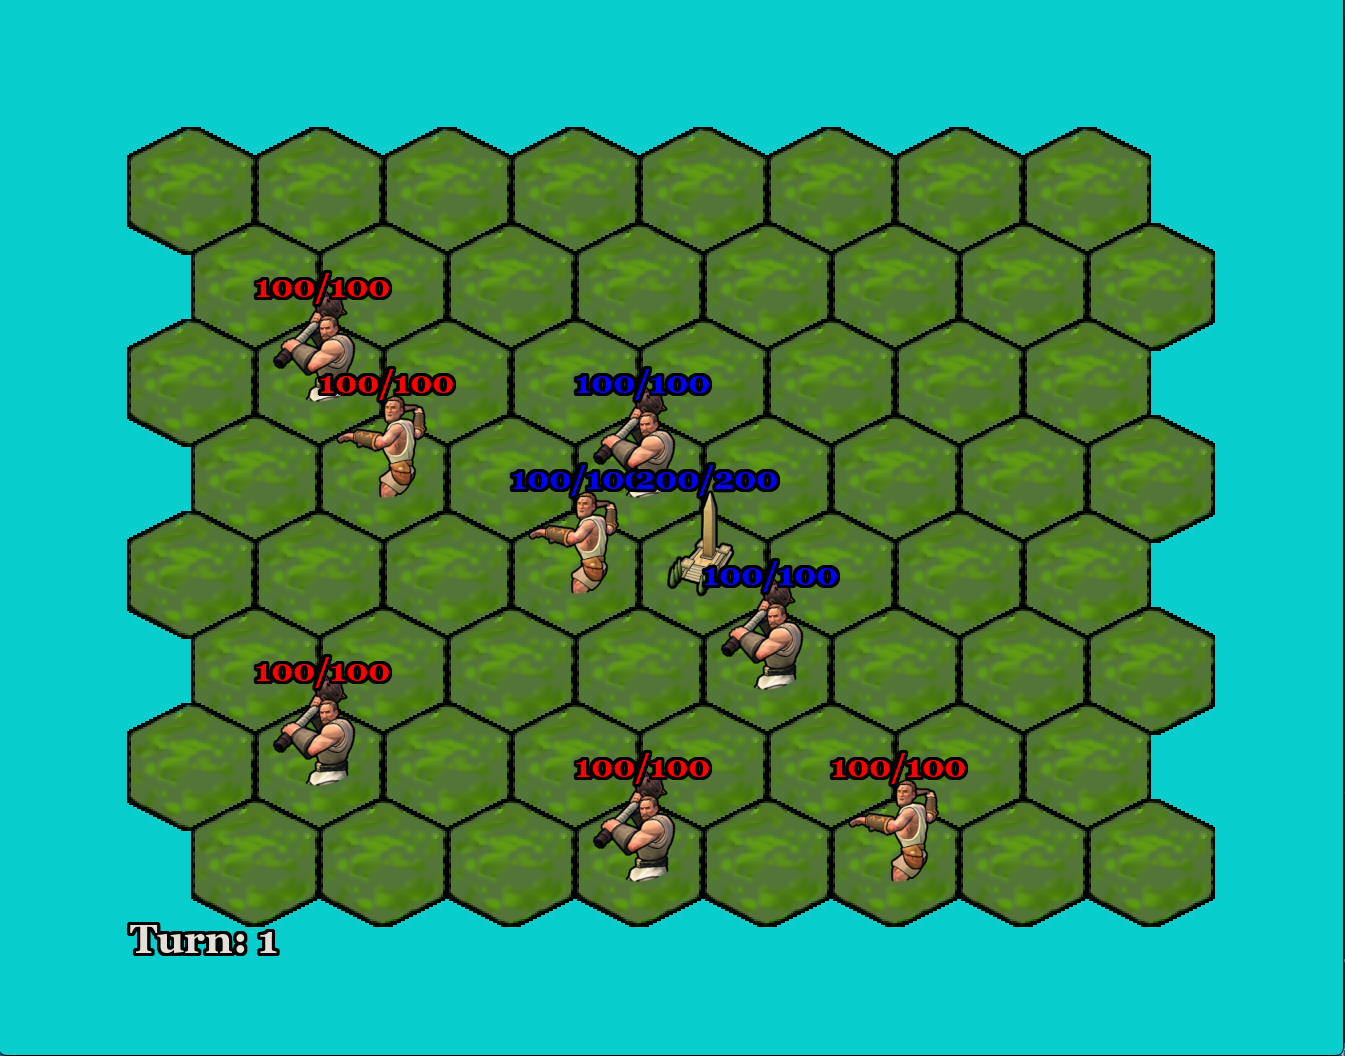
\includegraphics[scale=0.3]{gambar/environment_screenshot.png}
    % Keterangan gambar yang diinputkan
    \caption{\emph{Screenshot environment} dalam mode \emph{render}. \emph{Unit} milik agen \emph{attacker} memiliki teks \emph{hit points} berwarna merah dan unit milik agen \emph{defender} memiliki teks \emph{hit points} berwarna biru.}
    % Label referensi dari gambar yang diinputkan
    \label{fig:environmentScreenshot}
\end{figure}

\subsection{Unit dan Kota}
\emph{Unit} yang paling banyak jumlahnya dalam \emph{environment} ini adalah \emph{warrior}. 
\emph{Warrior} merupakan \emph{melee unit}, yang mana hanya dapat menyerang lawan yang berada di sebelah unit tersebut.
\emph{Warrior} memiliki attribut sebagai berikut:
\begin{itemize}
  \item HP: 100
  \item \emph{Movement Points}: 2
  \item \emph{Combat Strength}: 20
\end{itemize}

Jenis \emph{Unit} kedua adalah \emph{slinger}. \emph{Slinger} merupakan \emph{ranged unit} yang memiliki jarak sejauh 1 lantai.
\emph{Slinger} dapat menyerang \emph{unit} lain yang berdekatan dengan \emph{slinger} tanpa menerima \emph{damage} balasan dari \emph{unit} yang diserang.
\emph{Slinger} memiliki attribut sebagai berikut:
\begin{itemize}
  \item HP: 100
  \item \emph{Movement Points}: 2
  \item \emph{Combat Strength}: 5
  \item \emph{Ranged Strength}: 15
\end{itemize}

Kota merupakan tujuan utama yang perlu dihancurkan oleh agen \emph{attacker}. 
Kota akan berusaha melakukan perbaikan pada gilirannya dengan menambahkan +20 HP jika HP yang dimilikinya kurang dari nilai maksimum.
Kota tidak dapat melakukan perbaikan jika terdapat minimal tiga \emph{melee unit} milik agen \emph{attacker}.
Berikut adalah attribut dari kota:
\begin{itemize}
  \item HP: 200
  \item \emph{Combat Strength}: 28
\end{itemize}

\begin{figure}[!htb]
  \begin{minipage}{0.32\textwidth}
    \centering
    
\includegraphics[width=\linewidth]{gambar/warrior_1.png}
    \caption{\emph{Unit warrior}}\label{Fig:warrior}
  \end{minipage}\hfill
  \begin{minipage}{0.32\textwidth}
    \centering
    
\includegraphics[width=\linewidth]{gambar/slinger_1.png}
    \caption{\emph{Unit slinger}}\label{Fig:slinger}
  \end{minipage}
  \begin{minipage}{0.32\textwidth}
    \centering
    
\includegraphics[width=\linewidth]{gambar/city.png}
    \caption{Kota}\label{Fig:kota}
  \end{minipage}
\end{figure}

\subsection{Giliran dan Pergerakan Unit Agen}
Agen dapat mengkontrol \emph{unit} mereka pada giliran yang sudah ditentukan. 
\emph{Environment} dimulai dengan giliran agen \emph{attacker}, dilanjutkan oleh giliran kota, dan kemudian
ke giliran agen \emph{defender} sebelum kembali ke agen \emph{attacker}. 
Pergerakan dan pemilihan unit oleh agen dilakukan secara sekuensial. Pertama, agen akan memilih unit pertama mereka.
Agen akan melakukan pergerakan dengan unit yang telah dipilih sampai unit tersebut tidak lagi memiliki \emph{movement points}
pada giliran tersebut.
Setelah itu, agen akan berpindah ke unit selanjutnya. Hal ini akan berulang sampai agen tidak lagi memiliki unit yang masih
mempunyai \emph{movement points}. Jika agen sudah tidak memiliki unit yang masih mempunyai \emph{movement points}
maka agen akan mengakhiri giliran mereka dan giliran berikutnya akan dimulai. 
Sebuah \emph{episode} dari \emph{environment} akan berakhir ketika 20 giliran sudah berlalu, kota sudah hancur, atau seluruh \emph{unit}
milik agen \emph{attacker} mati.
Berikut flowchart dari pergerakan dan pemilihan sekuensial ini:

\begin{figure}[H]
  \centering
    % Nama dari file gambar yang diinputkan
    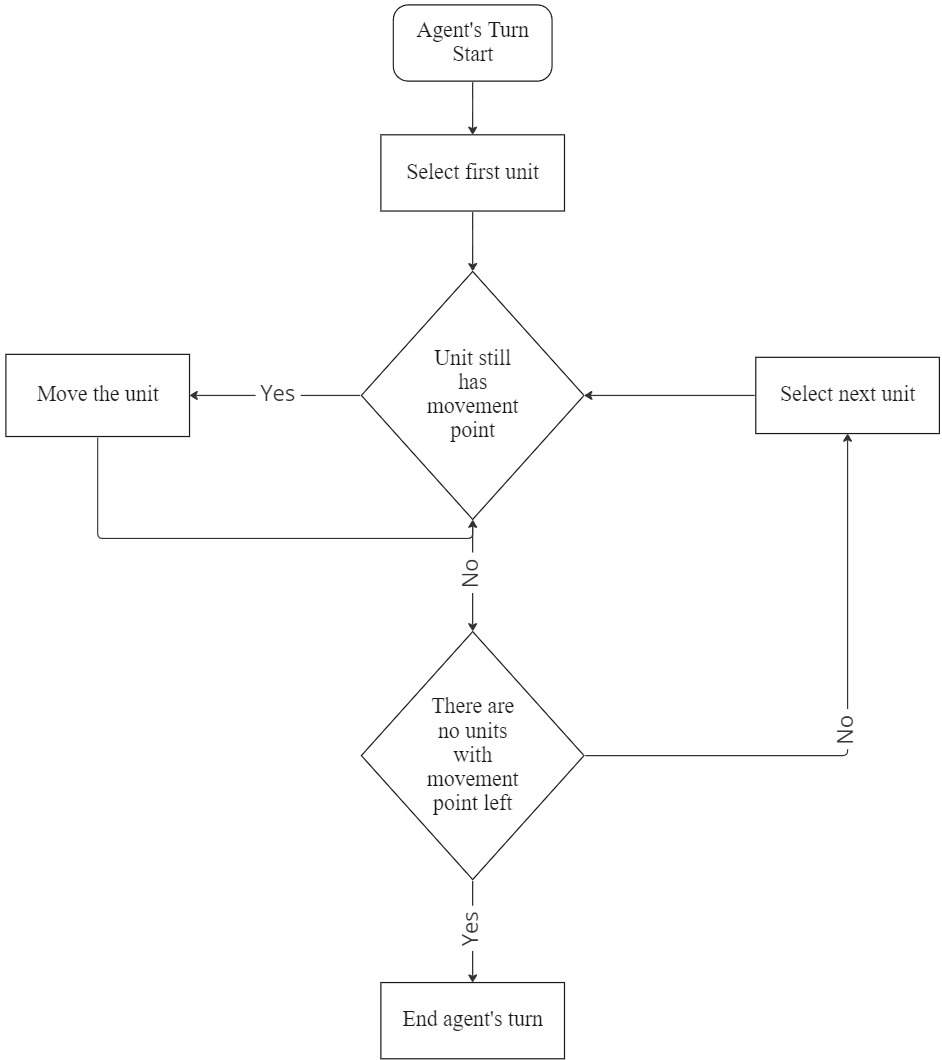
\includegraphics[scale=0.48]{gambar/unit_sequential_movement.jpg}
    % Keterangan gambar yang diinputkan
    \caption{\emph{Flowchart} pergerakan dan pemilihan sekuensial unit agen}
    % Label referensi dari gambar yang diinputkan
    \label{fig:sequentialMovementFlowchart}
\end{figure}

\subsection{Action Space}
\emph{Action space} merupakan kemungkinan yang dapat diambil oleh agen untuk melakukan sebuah \emph{action}.
\emph{Action space} yang digunakan dalam \emph{environment} ini adalah berupa 7 \emph{discrete actions}.
7 \emph{discrete actions} tersebut merupakan 6 sisi dimana unit dapat bergerak ke dan 1 \emph{action} unit tidak bergerak ke manapun.

% input gambar
\begin{figure}[H]
  \centering
    % Nama dari file gambar yang diinputkan
    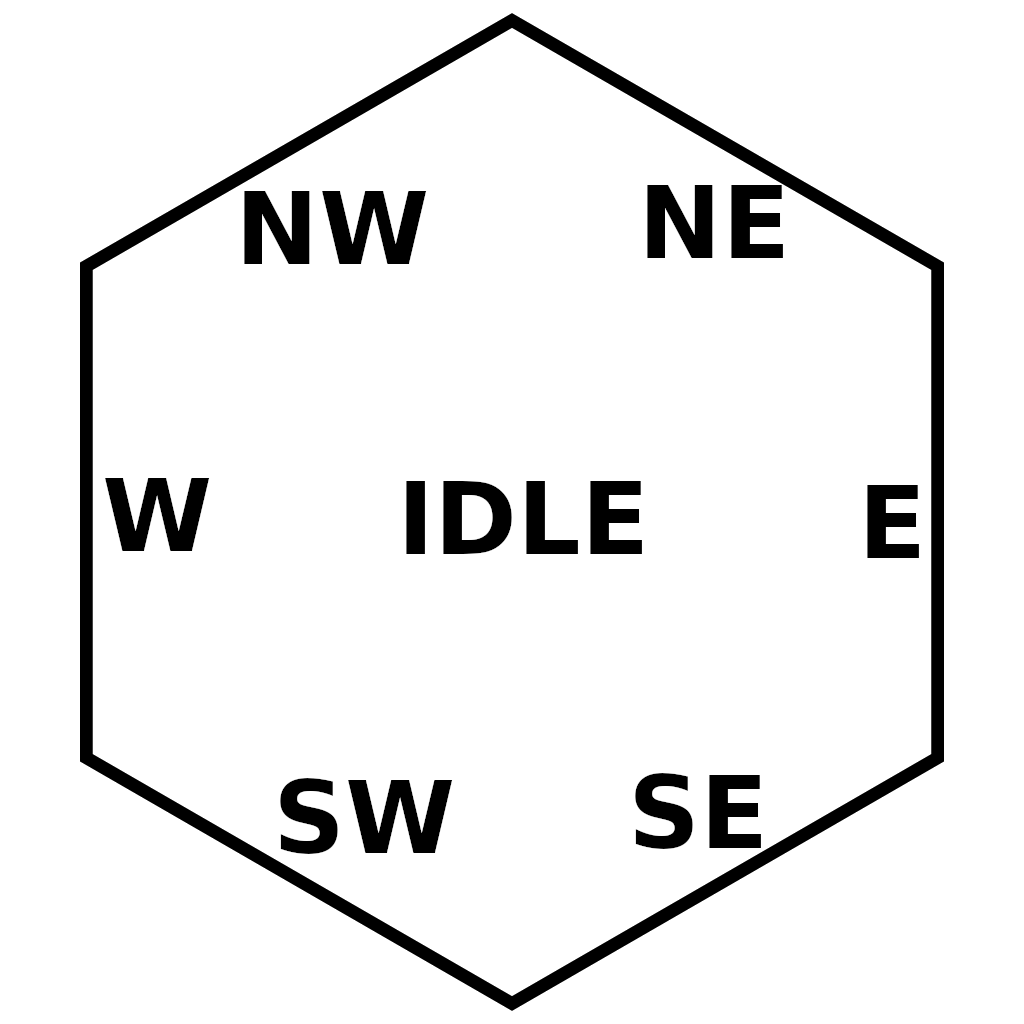
\includegraphics[scale=0.6]{gambar/hex_action.png}
    % Keterangan gambar yang diinputkan
    \caption{7 \emph{actions} yang dapat diambil oleh AI dalam \emph{Hexagonal tile}}
    % Label referensi dari gambar yang diinputkan
    \label{fig:hex_action}
\end{figure}

\subsection{Observation Space}
\emph{Observation Space} merupakan kumpulan \emph{state} dalam \emph{environment} yang didapatkan oleh agen saat melakukan observasi.
Agen dalam \emph{environment} penelitian ini melakukan \emph{complete observation}. 
Kedua agen mendapatkan informasi \emph{state} yang penuh dan sama saat melakukan observasi.
Seluruh nilai \emph{state} dinormalisasi sehingga nilainya berupa 0 sampai 1.
Berikut merupakan \emph{state} yang didapatkan oleh agen saat observasi:
\begin{itemize}
  \item Jarak seluruh unit dari kota: $x_{1}, y_{1}, \dots x_{n}, y_{n}$
  \item Nilai HP dari seluruh unit: $HP_{1}, \dots HP_{n}$
  \item Nilai movement points dari seluruh unit: $MP_{1}, \dots MP_{n}$
\end{itemize}

\subsection{Reward Agen}
\emph{Reward} merupakan nilai yang diberikan kepada agen ketika agen tersebut melakukan sebuah \emph{action}.
Karena \emph{environment} pada penelitian ini merupakan \emph{asymmetric}, maka terdapat dua tipe \emph{reward}:
\emph{general rewards} dan \emph{attacker rewards}. 
\emph{General rewards} adalah tipe \emph{reward} yang diberikan ke agen \emph{attacker} dan \emph{defender}.
Sedangkan \emph{attacker rewards} hanya diberikan pada agen \emph{attacker}.
Berikut \emph{reward} tersebut:
\begin{itemize}
  \item General rewards: \begin{itemize}
      \item Bergerak ke luar batas \emph{environment} = -1
      \item Melakukan \emph{healing} pada sebuah \emph{unit} = +0.1
      \item Menyerang \emph{unit} lawan = +0.2
      \item Mematikan \emph{unit} lawan = +3
  \end{itemize}
  \item Attacker rewards: \begin{itemize}
      \item Menghancurkan kota = +20
      \item Menyerang kota = +0.5
      \item Kota melakukan perbaikan = -0.3
      \item Sebuah \emph{unit} mati = -1
      \item Sebuah giliran telah berlalu = -1
  \end{itemize}
\end{itemize}

Agen \emph{attacker} akan mendapatkan +20 poin ketika menghancurkan kota, karena itu merupakan tujuan utama dari agen \emph{attacker}.
Jika sebuah \emph{unit} agen \emph{attacker} mati atau sebuah giliran telah berlalu maka agen \emph{attacker} akan mendapatkan -1 point
Hal ini untuk memaksa agen \emph{attacker} agar menyelesaikan tujuannya secepat mungkin dan meminimalisir kehilangan \emph{unit}.

Agen \emph{defender} yang memiliki tujuan untuk mencoba mencegah agen \emph{attacker} mendapatkan +3 poin ketika sebuah \emph{unit}
agen \emph{attacker} mati. Tidak diberikan penalti pada agen \emph{defender} ketika unit mereka mati karena pada eksperimen sebelumnya,
hal tersebut membuat agen \emph{defender} terlalu pasif. Kedua agen akan mendapatkan penalti ketika mencoba untuk menggerakan \emph{unit}
milik mereka keluar dari batas \emph{environment}.


% % Per blok diagram dijelaskan dan dibuatkan section masing-masing

% % \section{Blok Diagram}
% % \label{sec:blokdiagram}

% % Contoh pembuatan potongan kode
% \begin{lstlisting}[
%   language=C++,
%   caption={Program halo dunia.},
%   label={lst:halodunia}
% ]
% #include <iostream>

% int main() {
%     std::cout << "Halo Dunia!";
%     return 0;
% }
% \end{lstlisting}

% \lipsum[2-3]

% % Contoh input potongan kode dari file
% \lstinputlisting[
%   language=Python,
%   caption={Program perhitungan bilangan prima.},
%   label={lst:bilanganprima}
% ]{program/bilangan-prima.py}

% \lipsum[4]
